\documentclass[12pt]{scrartcl}
\usepackage[german, ngerman]{babel}
\usepackage{graphicx}
\usepackage{color}
\usepackage{url}
\usepackage{xcolor}
\usepackage{listings}
\usepackage{hyperref}
\usepackage{nameref}
\usepackage{varioref}
\hypersetup{
    colorlinks=true,
    linkcolor={black!50!black},
    % linkcolor={red!50!black},
    citecolor={black!50!black},
    urlcolor={black!50!black}
}
\usepackage[headsepline,footsepline]{scrlayer-scrpage}
\usepackage{biblatex}
\usepackage{amsmath}
\usepackage{float}
\usepackage{multirow}


\newcommand{\code}[1]{\texttt{#1}}


\definecolor{mGreen}{rgb}{0,0.6,0}
\definecolor{mGray}{rgb}{0.5,0.5,0.5}
\definecolor{mPurple}{rgb}{0.58,0,0.82}
\definecolor{backgroundColour}{rgb}{0.95,0.95,0.95} %{cmyk}{0.05,0.05,0.05,0.05}

\lstdefinestyle{CStyle}{
    backgroundcolor=\color{backgroundColour},
    commentstyle=\color{mGreen},
    keywordstyle=\color{blue},
    numberstyle=\tiny\color{mGray},
    stringstyle=\color{mPurple},
    basicstyle=\footnotesize,
    breakatwhitespace=false,
    breaklines=true,
    captionpos=b,
    keepspaces=true,
    numbers=left,
    numbersep=5pt,
    showspaces=false,
    showstringspaces=false,
    showtabs=false,
    tabsize=2,
    language=C++
}

\lstdefinestyle{Terminal}{
    backgroundcolor=\color{backgroundColour},
    commentstyle=\color{black},
    keywordstyle=\color{black},
    numberstyle=\tiny\color{black},
    stringstyle=\color{black},
    basicstyle=\footnotesize,
    breakatwhitespace=false,
    breaklines=true,
    captionpos=b,
    keepspaces=true,
    numbers=none,
    numbersep=5pt,
    showspaces=false,
    showstringspaces=false,
    showtabs=false,
    tabsize=2,
}


\pagestyle{scrheadings}
\clearscrheadfoot
%\cfoot{Tobias Gruber}
\cfoot{\pagemark}
\chead{\headmark}
\automark[subsection]{section}


\begin{document}


\begin{titlepage}
    \vfill
	\centering
    \vspace{1.5cm}

	{\scshape\LARGE Hochschule München \par}
    {\scshape\Large Fakultät für Informatik und Mathematik\par}
	\vspace{1.5cm}




    \vfill
    {\LARGE\bfseries Praktikumsaufgabe 4 \\}
    \vspace{0.5cm}
	{in der Vorlesung\\}
    \vspace{0.5cm}
    {\LARGE\bfseries Computational Geometry\\~\\ \par}
	{\LARGE Konvexe Hüllen mit qhull\\~\\ \par}
	\vfill
    \vfill


    \begin{tabular}{ll}
    \normalsize
    Team:  & Christopher Hinz, Tobias Gruber\\
    Studiengruppe: & Master Informatik\\
    Studiensemester: & 1. Semester\\
    Schwerpunkt: & Embedded Computing\\
    \end{tabular}
    \vspace{1.5cm}

    \today

    \vspace{0.5cm}

    Sommersemester 2022

	\vfill

\end{titlepage}

\newpage

%%%%%%%%%%%%%%%%%%%%%%%%%%%%%
% Einführung
%%%%%%%%%%%%%%%%%%%%%%%%%%%%%
\section{Einführung}
Im Zuge dieses Praktikum wird das Programm qhull zur Erzeugung von Punktmengen und Berechnung konvexer Hüllen verwendet. Hierbei ist das Ziel die Ausgaben des Programms nachzuvollziehen und zu verstehen.


%%%%%%%%%%%%%%%%%%%%%%%%%%%%%
% Funktionen von qhull
%%%%%%%%%%%%%%%%%%%%%%%%%%%%%
\section{Funktionen von qhull}

Qhull bietet 6 verschiedene Programme an:
\begin{itemize}
    \setlength\itemsep{0em}
    \item qconvex: convex hulls
    \item qdelaunay: Delaunay triangulations and furthest-site Delaunay triangulations
    \item qhalf: halfspace intersections about a point
    \item qhull: all structures with additional options
    \item qvoronoi: Voronoi diagrams and furthest-site Voronoi diagrams
    \item rbox: generate point distributions for qhull
\end{itemize}

Im Zuge dieses Praktikums werden wir sowohl rbox, zur Erzeugung von Punktmengen nutzen, als auch qconvex, zur Berechnung der konvexe Hüllen.
Qhull nutzt hierbei den, in der Vorlesung besprochenen, Quick Hull Algorithmus. Dieser teilt für die Berechnung der konvexen Hülle die Punktmengen nach dem "divide and conquer" Prinzip auf. Hierbei dienen jeweils die Extrempunkte (z.B maximaler und minimaler x-Wert für erste Teilung) als Kriterien zur Teilung der Punktmenge. Als Ergebnis des Algorithmus erhält man die Hyperebenen, die die konvexe Hülle bilden.



\subsection{rbox}
Das Programm rbox generiert zufällige oder reguläre Punkte. Diese dienen als Datensatz über den die konvexe Hülle berechnet werden soll.
Einige Beispiele zur Erzeugung von Punktmengen sind:
\begin{itemize}
    \setlength\itemsep{0em}
    \item rbox 10 D3: erzeugt 10 Punkte in 3D
    \item rbox 15 D4: erzeugt 15 Punkte in 4D
    \item rbox 10 D2: erzeugt 10 Punkte auf einem 2D Kreis
    \item rbox 100 W0: erzeugt 100 Punkte  auf der Oberfläche eines Würfels
\end{itemize}
\newpage

\subsection{Beispiele}
Bevor auf Details von qconvex eingegangen wird, sollen zwei kurze Beispiele die Eingabedaten und die Ergebnisse der Berechnung visualisieren.\\
Zur Demonstration der Funktion von qconvex sollen Zufallsdaten und deren konvexe Hülle visualisiert werden. Hierzu wurde ein Python-Skript implementiert das die Datenpunkte plottet und aus den Ergebnissen von qconvex die Hyperebenen zeichnet. 

\ \\
\underline{Punkte und konvexe Hülle in 2 Dimensionen}\\~\\
Im erste Beispiel werden die Datenpunkte in 2 Dimensionen erzeugt und eingelesen und deren Hyperebenen (Geraden) mit qconvex berechnet. Der nachfolgende Plot zeigt dies:
\begin{figure}[H]
    \centering
    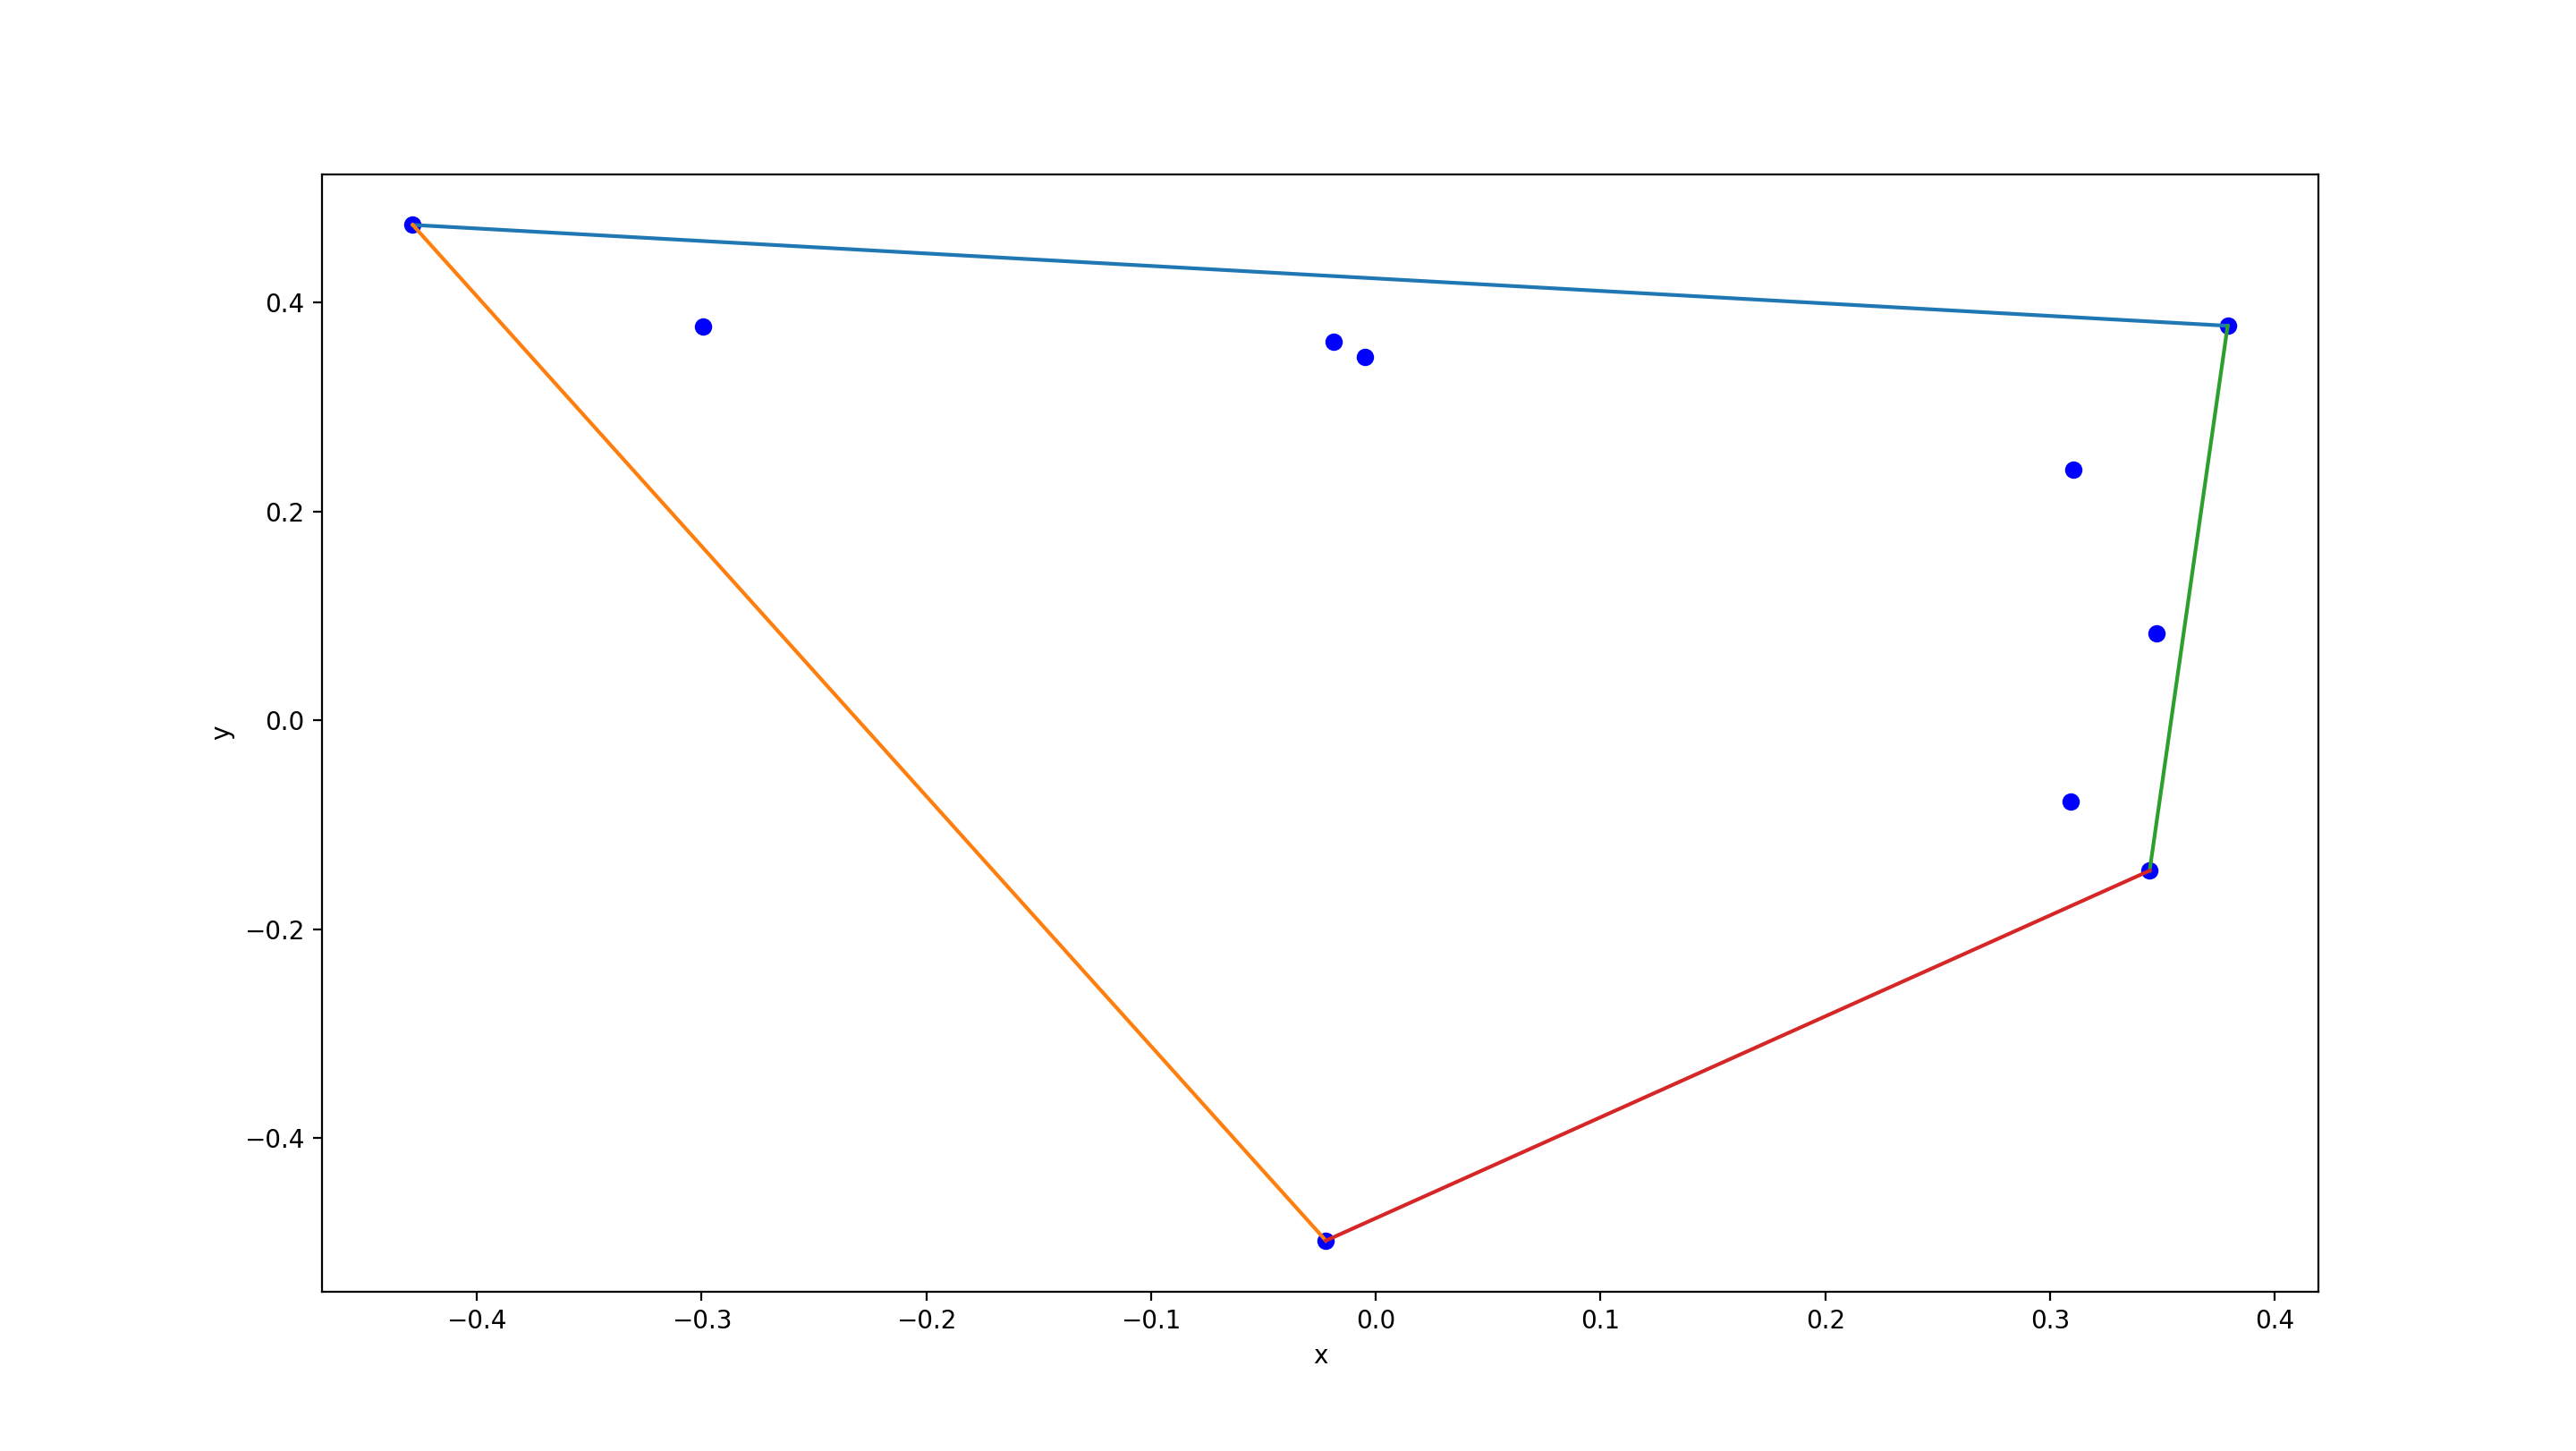
\includegraphics[scale=0.3]{2D_plot.png}
\end{figure}
\ \\
\underline{Punkte und konvexe Hülle in 3 Dimensionen}\\~\\
Im zweiten Beispiel werden die Datenpunkte in 3 Dimensionen erzeugt und eingelesen und ebenfalls die Hyperebenen (Ebenen) mit qconvex berechnet. Auch dies ist untenstehend mit matplotlib visualisiert:
\begin{figure}[H]
    \centering
    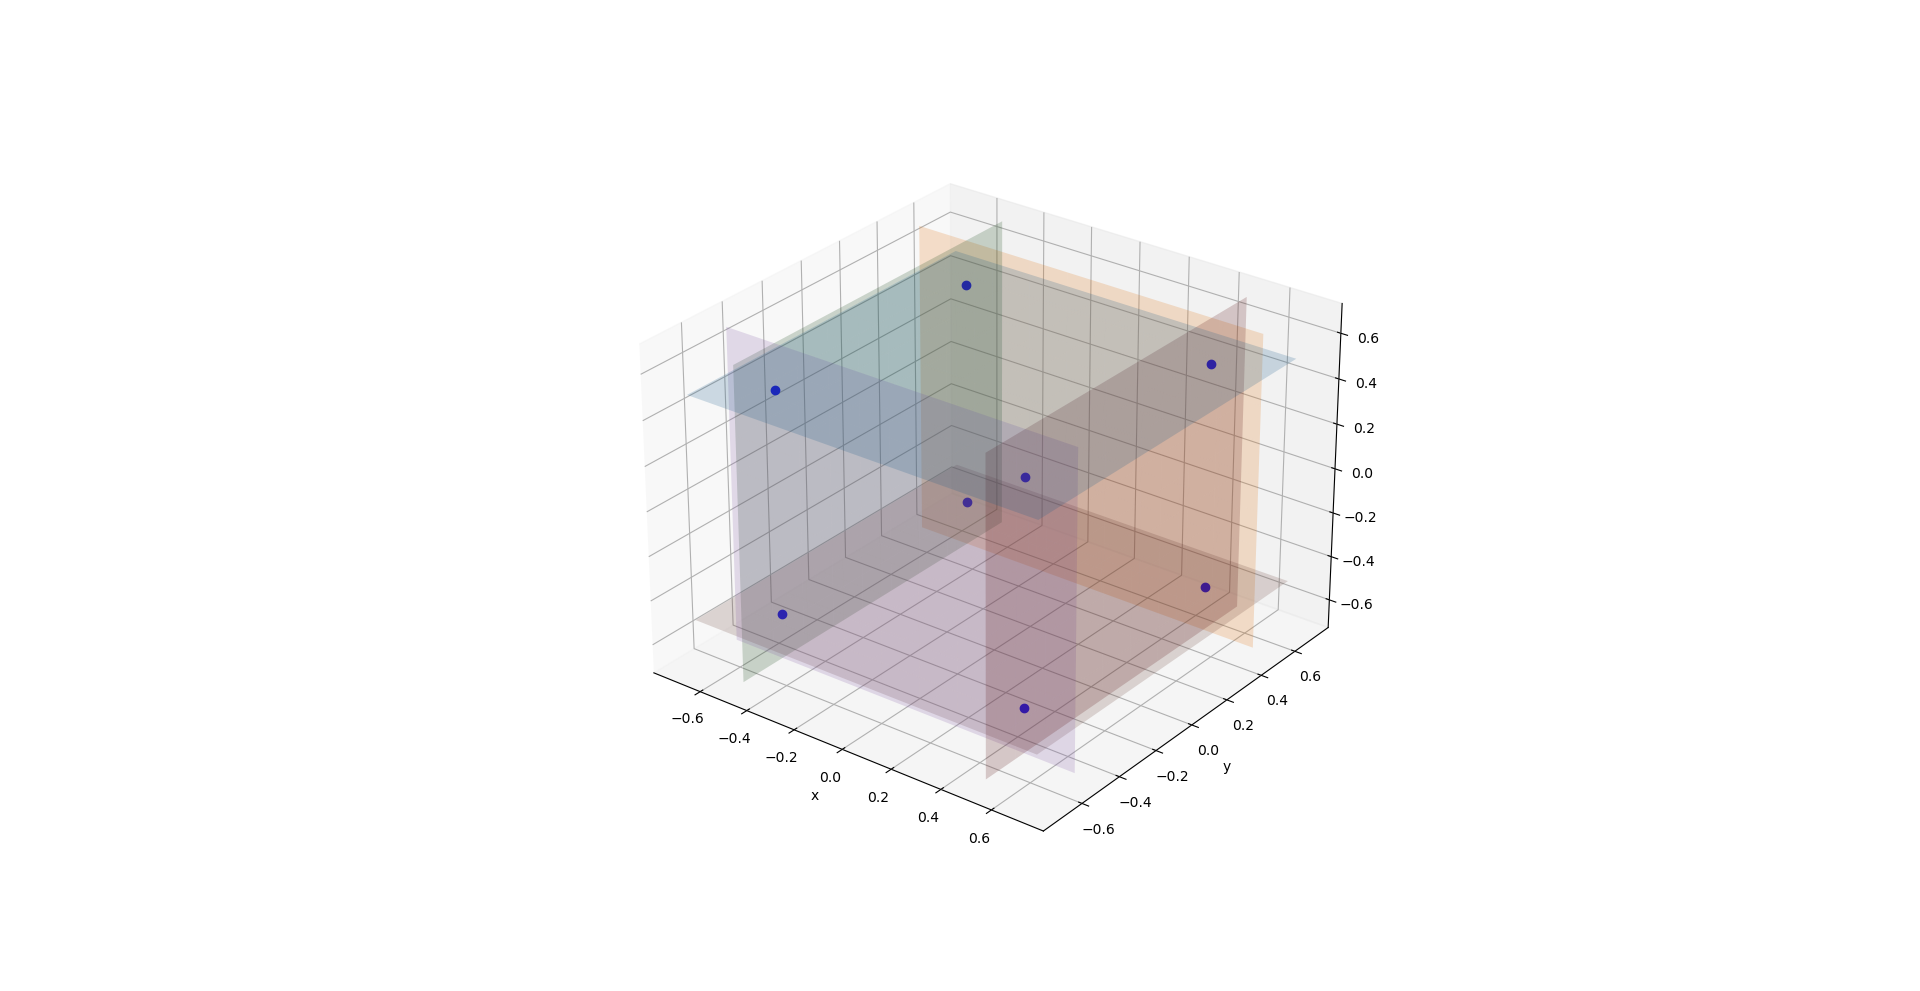
\includegraphics[scale=0.3]{cubeplot.png}
\end{figure}

\subsection{Zeitmessung}
Es soll die Laufzeit des Algorithmus für verschiedene Punktmengen in unterschiedlichen Dimensionen gemessen werden.  Eine Zeitangabe ist bei der Ausgabe der Zusammenfassung des Ergebnisses enthalten. Die Zusammenfassung erhält man durch die qconvex Option 's'. Das Ergebnis der Messungen ist untenstehend grafisch und tabellarisch dargestellt.
\begin{center}
\begin{tabular}{||c | c c c c c c c||} 
    \hline
    Dimension & 2D &       3D &      4D &       5D &       6D &       7D &       8D      \\
    \hline \hline
    \multirow{4}{*}{Laufzeit in s} & 2.3e-05 &  3.4e-05 & 3.5e-05 &  4.2e-05 &  5.8e-05 &  6.2e-05 &  4.8e-05 \\ \cline{2-8}
                                   & 3e-05 &    6.3e-05 & 0.000186 & 0.000832 & 0.003005 & 0.009608 & 0.03245 \\ \cline{2-8}
                                   & 3.6e-05 &  7.8e-05 & 0.000298 & 0.001947 & 0.009298 & 0.04809 &  0.2151  \\ \cline{2-8}
                                   & 0.000116 & 0.00021 & 0.000907 & 0.007799 & 0.06736 &  0.876 &    9.933   \\ \hline
\end{tabular}
\end{center}

\begin{figure}[H]
    \centering
    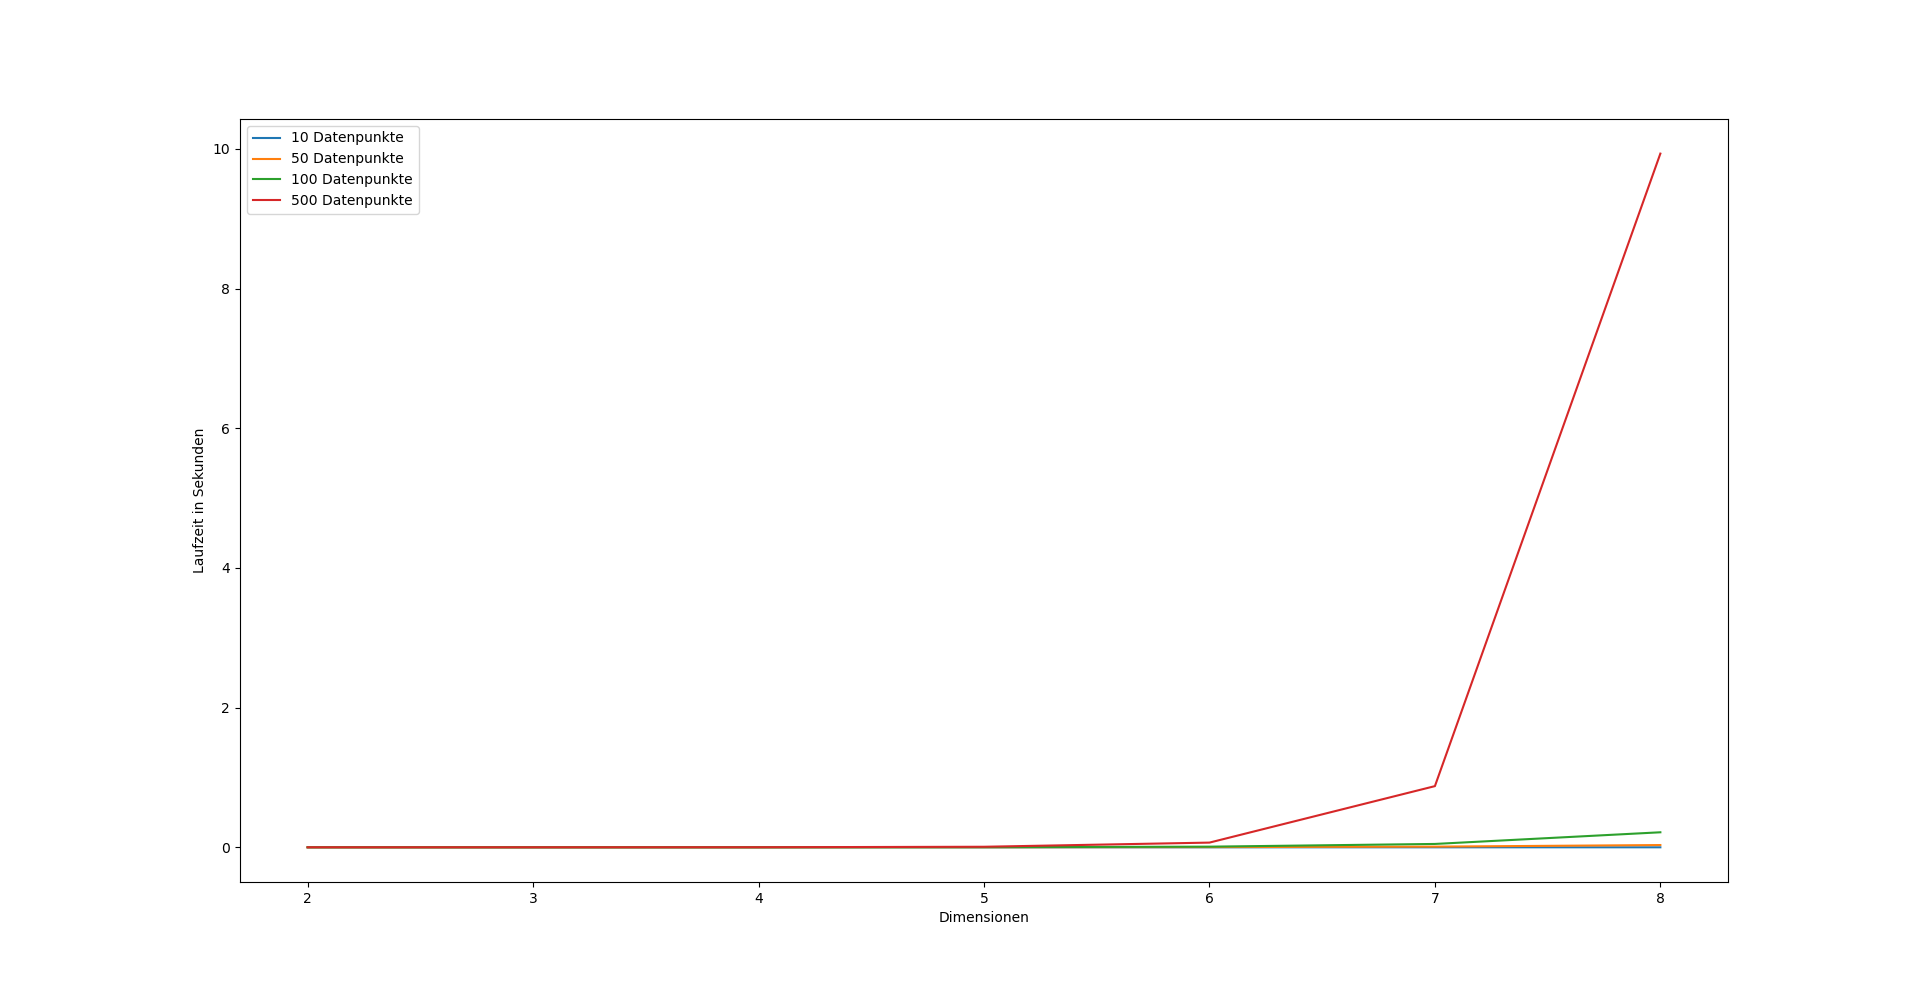
\includegraphics[scale=0.32]{runtimes.png}
\end{figure}

\ \\ 
Zusätzlich soll die Komplexität des Quick Hull Algorithmus in 2 Dimensionen untersucht werden.
Die Komplexität ist mit $\Omega(n*log(k))$ gegeben. Damit hängt die Komplexität neben der Anzahl der Punkte auch von der Anzahl der berechneten Kanten ab.  
Das foldende Bild zeigt die Laufzeiten für zunehmende Punktzahlen. Es ist gut zu erkennen, dass ein annähernd linearer Zusammenhang besteht. Dies lässt sich darauf zurückführen, dass die Anzahl der Kanten nicht proportional mit der Anzahl der Punkte wächst und auch für hohe Punktzahlen eine geringe Anzahl an Kanten berechnet werden (z.B. 28 Kanten für 50 Punkte und 46 Kanten bei 1.000.000 Punkten). Dadurch ist der Ausdruck $log(k)$ annhähernd konstant und der Verlauf der Kurve hängt insbesondere von n ab und ist damit linear.


\begin{figure}[H]
    \centering
    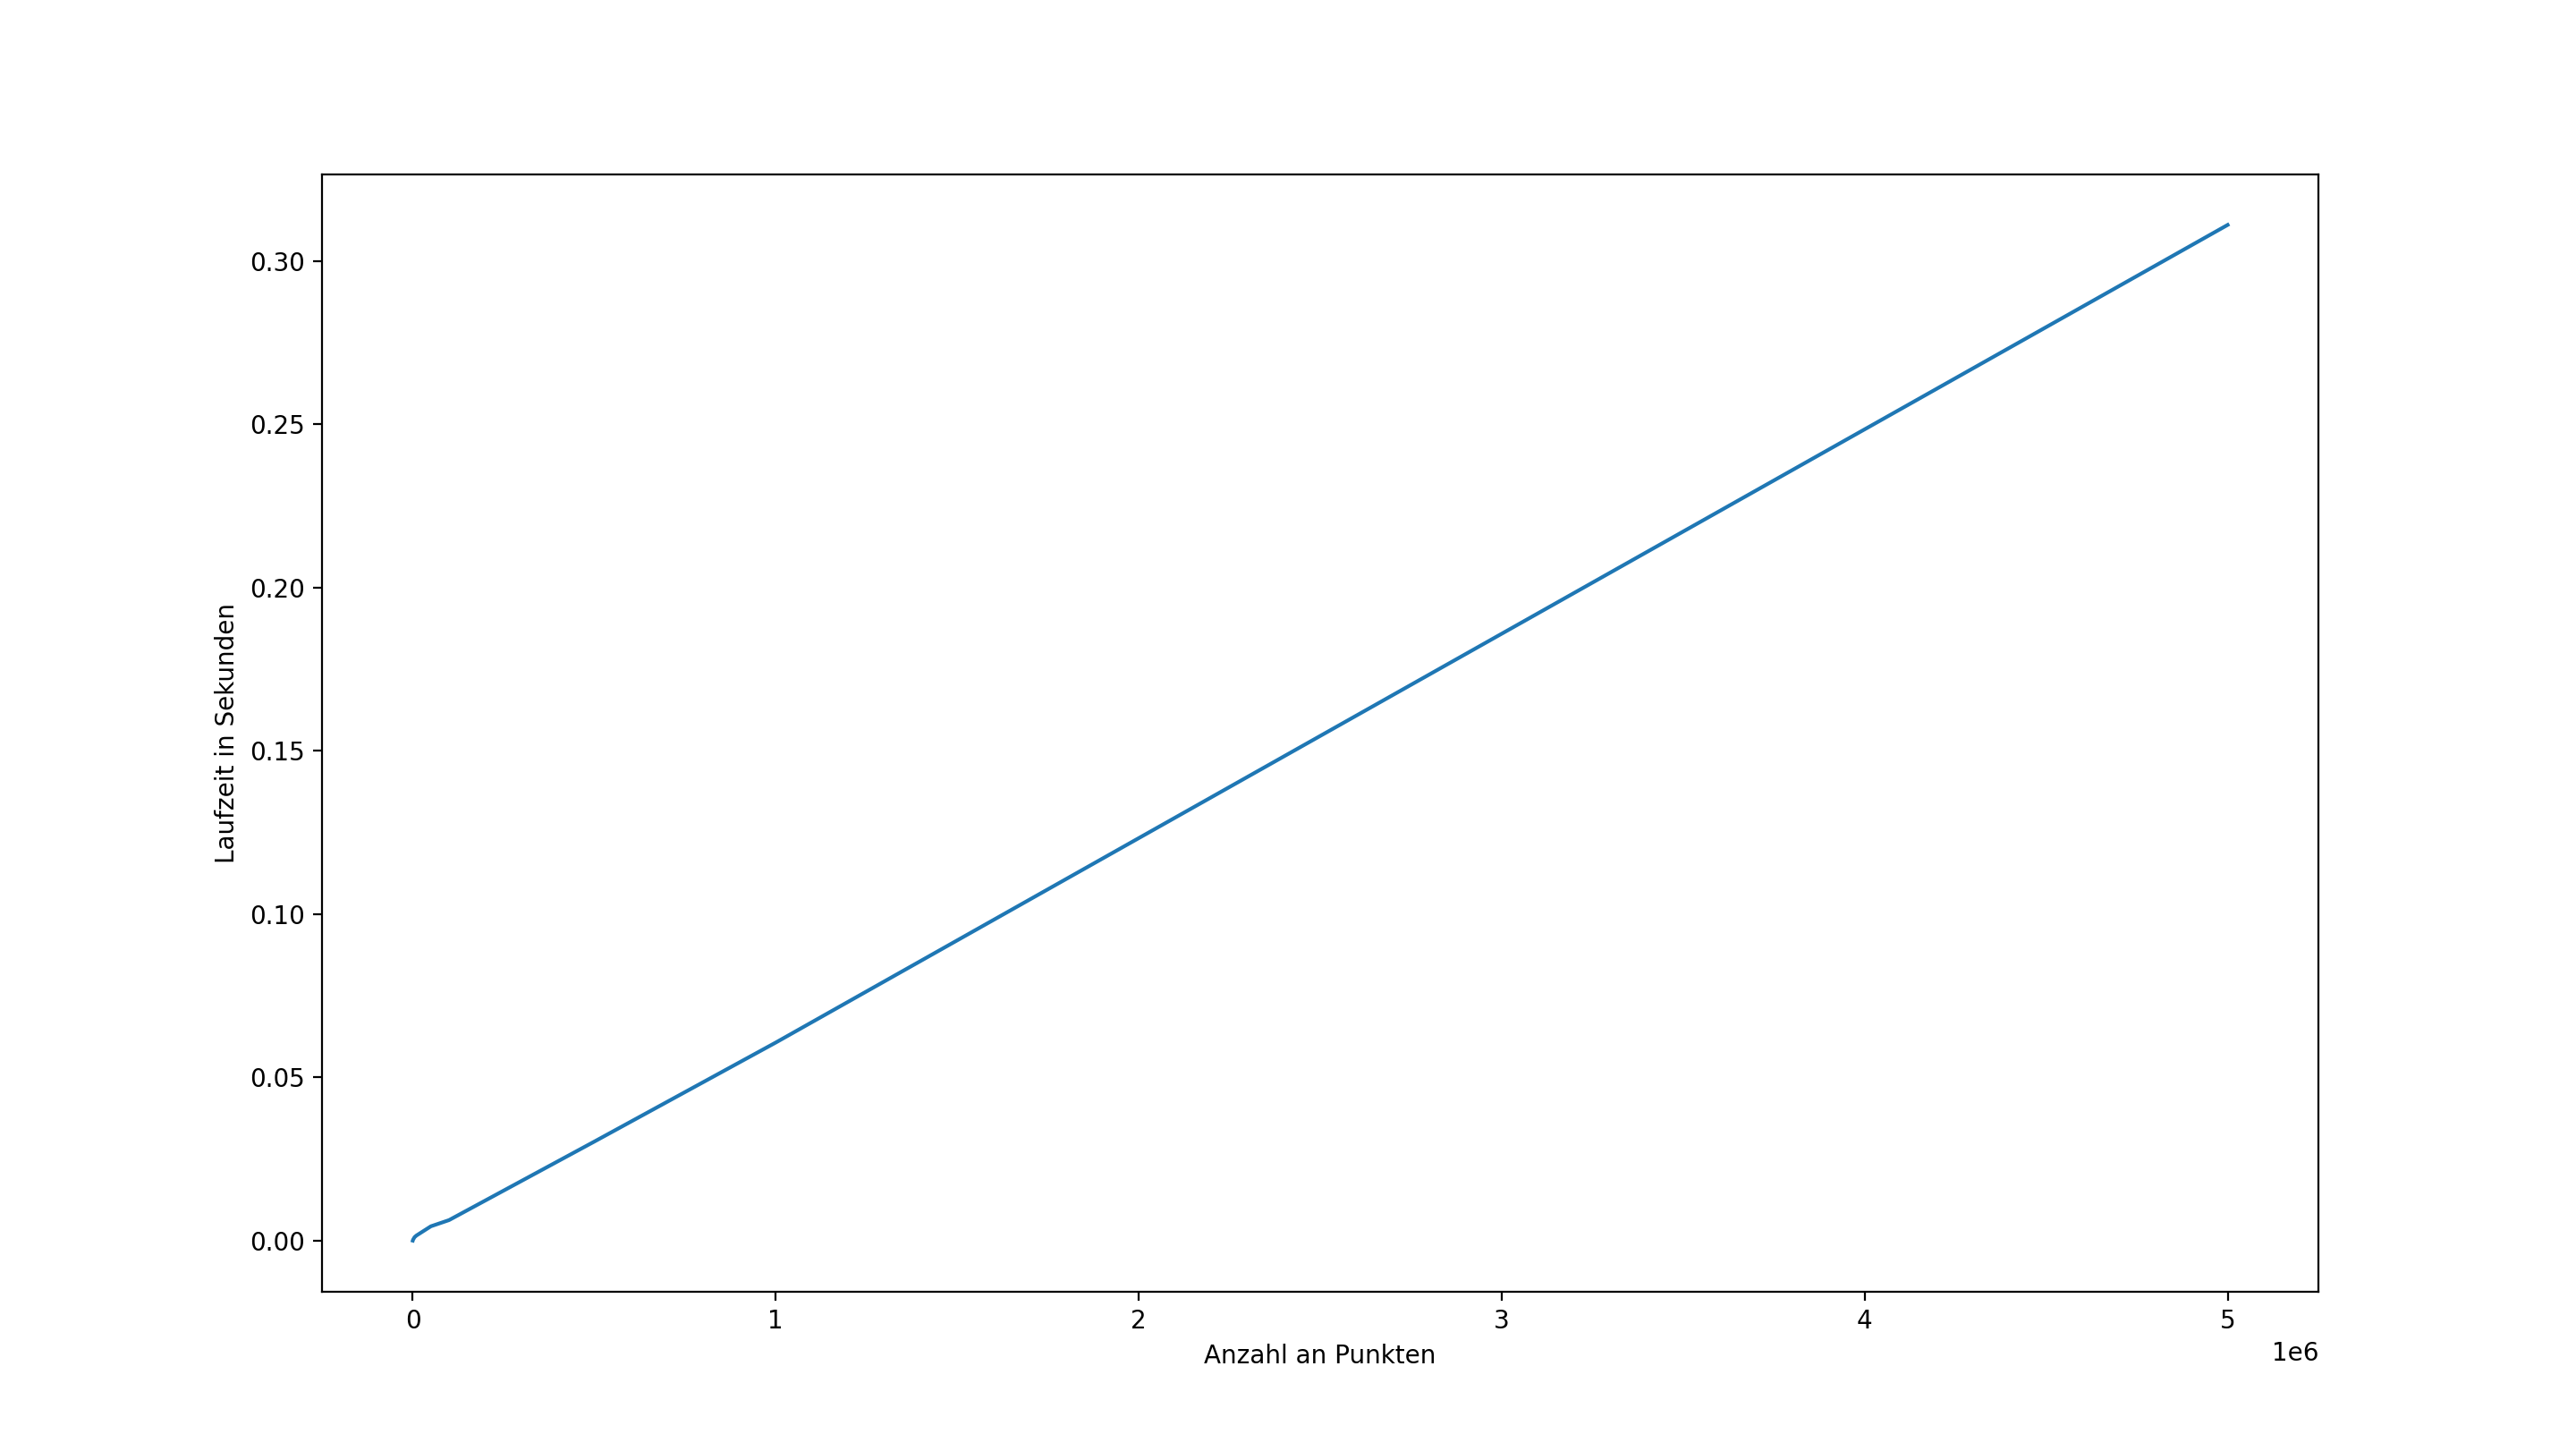
\includegraphics[scale=0.32]{runtimes2.png}
\end{figure}



\subsection{qconvex}
Im Folgenden sollen die Ausgaben bzw. die Ergebnisse von qconvex genauer betrachtet werden. Die bereits erwähnt stellt qconvex Informationen über die Hyperebenen der konvexen Hülle über eine Punktmengen bereit. Wie diese Informationen ausgegeben und interpretiert werden müssen soll nachfolgend genauer betrachtet werden.

\ \\
\underline{Normalenvektoren der Hyperebenen}\\~\\
Eine mögliche Ausgabe von qconvex sind die Normalenvektoren der Hyperebenen, also in der Hesseschen Normalenform. Die Normalenvektoren können über die Option 'n' ausgegeben werden. Für jede berechnete Hyperebene erhält man jeweils den Normalenvektor und den Abstand der Hyperebene vom Ursprung. Mit Hilfe dieser Parametern lassen sich die Hyperebenen darstellen.\\~\\

In 2 Dimensionen erhält man 3 Parameter pro Hyperebene (Gerade). Die zwei ersten sind die Koordinaten des Normalenvektors, der dritte entspricht dem Abstand zum Ursprung. Diese repräsentieren die Parameter der Hesseschen Normalenform wie folgt:\\

$ g: n_1*x+n_2*y+d = 0 $ mit Normalenvektor: $\vec{n} = \begin{pmatrix}n_1 \\ n_2\end{pmatrix}, d \widehat{=} Abstand$

\ \\

Für oben gezeigte Beispiel in zwei Dimensionen erhält man die folgende Ausgabe:
\begin{lstlisting}[style=Terminal, caption={Ausgabe von qconvex mit Option 'n'},captionpos=b]
        0.1187746524595787 0.9929212365203528 -0.4203231200255335 
        -0.9227096915324942 -0.3854955578888162 -0.2124714536362973 
        0.9977929883946747 -0.06640144810487485 -0.3530963274142334 
        0.6949453872092842 -0.7190625207842071 -0.3426299574618282 
\end{lstlisting}

 
Hieraus lassen sich nun die 4 Geradengleichungen aufstellen:
\begin{itemize}
    \item $g_1: 0.1187746524595787*x + 0.9929212365203528*y - 0.4203231200255335 = 0 $
    \item $g_2: -0.9227096915324942*x - 0.3854955578888162*y - 0.2124714536362973 = 0 $
    \item $g_3: 0.9977929883946747*x - 0.06640144810487485*y - 0.3530963274142334 = 0 $
    \item $g_4: 0.6949453872092842*x - 0.7190625207842071*y - 0.3426299574618282 = 0 $
\end{itemize}


In 3 Dimensionen erhält man entsprechend 4 Parameter pro Hyperebene (Ebene). Die drei ersten sind die Koordinaten des Normalenvektors, der vierte entspricht dem Abstand zum Ursprung. Diese entsprechen den Parametern einer Ebene in der Hesseschen Normalenform:\\

$ e: n_1*x+n_2*y+n_3*z+d = 0 $ mit Normalenvektor: $\vec{n} = \begin{pmatrix}n_1 \\ n_2 \\ n_3\end{pmatrix}, d \widehat{=} Abstand$

\ \\
Auch hier können analog zum Vorgehen in 2 Dimensionen alle Ebenengleichungen aufgestellt werden.\\
Das selbe gilt auch für alle höheren Dimensionen. Auch hier entspricht der letzte Parameter der Ausgabe jeweils dem Abstand zum Ursprung und alle weiteren Parameter sind die Koordinaten des Normalenvektors.\\

\ \\
\underline{Punkte der Hyperebenen}\\~\\
Eine weitere mögliche Ausgabe sind die Koordinaten der Punkte welche die Hyperebene aufspannen. Diese können über die Option 'o' ausgegeben werden. Die Ausgabe besteht hier aus einem Teil der bestimmte Vertices definiert und einem Teil der die Vertices den Facetten/Hyperebenen zuordnet. Die entsprechende Ausgabe für das Beispiel in 2 Dimensionen sieht folgendermaßen aus:

\begin{lstlisting}[style=Terminal, caption={Ausgabe von qconvex mit Option 'o'},captionpos=b]
    -0.02222276248244826 -0.4979727817680433    // Index 0
    -0.4285431913366012 0.4745826469497594      // Index 1
    0.3105396575392593 0.2400179190933871       // ...
    -0.01883958887200765 0.3630260628303755 
    0.3790312361708201 0.3779794437605696 
    -0.2994955874043476 0.3776609263174803 
    0.3471817493878135 0.08365533089605659 
    -0.00485819764887746 0.3482682405489201 
    0.3443122672329771 -0.1437312230875075 
    0.309330780347186 -0.07758103877080702 
    2 4 1 
    2 1 0 
    2 8 4 
    2 0 8 
\end{lstlisting}
\ \\
Der untere Teil gibt als erstes die Anzahl an Vertices an, gefolgt von der Nummer bzw. Index des entprechendem Vertex. So bedeutet die erste Zeile, dass die 2 Vertices der ersten Hyperebene durch eine Gerade durch die Punkten 4 und 1 definiert ist.\\
Damit ist jede Gerade in der folgenden Form definiert:\\~\\
$ \vec{x} = \vec{s} + \lambda * (\vec{t}-\vec{s})$ mit $\vec{s} = \begin{pmatrix} s_1 \\ s_2 \end{pmatrix}, \vec{t} = \begin{pmatrix} t_1 \\ t_2 \end{pmatrix}$
\ \\
In drei Dimensionen ist die Ebene durch drei Punkte aufgespannt und ist definiert durch:\\~\\
$ \vec{x} = \vec{s} + \lambda_1 * (\vec{t}-\vec{s}) + \lambda_1 * (\vec{r}-\vec{s})$ mit $\vec{s} = \begin{pmatrix} s_1 \\ s_2 \\ s_3 \end{pmatrix}, \vec{t} = \begin{pmatrix} t_1 \\ t_2 \\ t_3\end{pmatrix}, \vec{r} = \begin{pmatrix} r_1 \\ r_2 \\ r_3 \end{pmatrix}$
\ \\~\\~\\
Das selbe gilt auch hier wieder analog für höhere Dimensionen.\\


\ \\
\underline{Kombinierte Information der Hyperebenen}\\~\\
Die letzte zu erwähnende Option stellt beide oben erwähnten Repräsentationen der Hyperebenen zusammen und formatiert dar. Zur Ausgabe wird die qconvex Option 'f' genutzt:\\

\begin{lstlisting}[style=Terminal, caption={Ausgabe von qconvex mit Option 'f'},captionpos=b]
    Vertices and facets:
    - p4(v2):  0.38  0.38
    - p1(v1): -0.43  0.47
    - p0(v3): -0.022  -0.5
    - p8(v4):  0.34 -0.14
    - f1
        - flags: top simplicial
        - normal:    0.1188   0.9929
        - offset: -0.4203231
        - vertices: p4(v2) p1(v1)
        - neighboring facets: f2 f4
    - f2
        - flags: bottom simplicial
        - normal:   -0.9227  -0.3855
        - offset: -0.2124715
        - vertices: p0(v3) p1(v1)
        - neighboring facets: f1 f5
    - f4
        - flags: top simplicial
        - normal:    0.9978  -0.0664
        - offset: -0.3530963
        - vertices: p8(v4) p4(v2)
        - neighboring facets: f1 f5
    - f5
        - flags: bottom simplicial
        - normal:    0.6949  -0.7191
        - offset:   -0.34263
        - vertices: p8(v4) p0(v3)
        - neighboring facets: f2 f4
\end{lstlisting}
\ \\
Auch hier sind die Informationen über die Hyperebene als Punkte der Hyperebene und als Normalenvektoren und Abstand gegeben.




\end{document}

